\subsection{Metodo Delphi}

El método \textbf{Delphi} es una técnica de pronóstico que busca el consenso de un grupo de expertos. Se basa en rondas de cuestionarios anónimos, donde la retroalimentación gradual converge hacia un acuerdo. Para el proyecto ``SafeSight'', se aplicó para evaluar y refinar una propuesta de sistema de control de acceso escolar con reconocimiento facial, asegurando una solución robusta y adaptada a la comunidad educativa.

\begin{figure}[H]
    \centering
    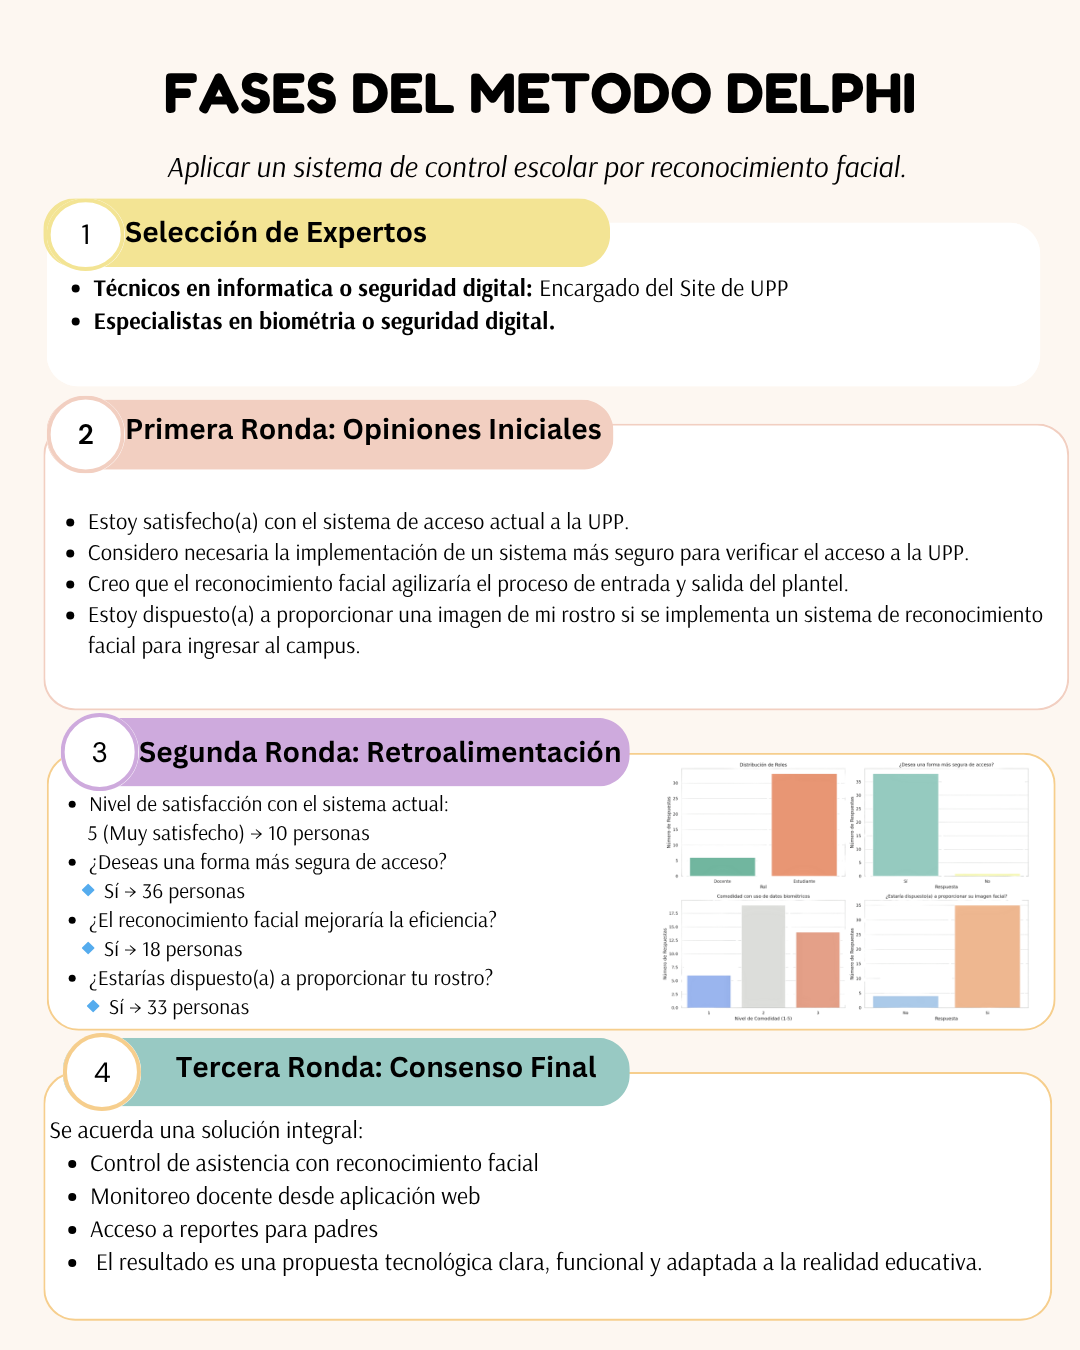
\includegraphics[width=0.85\textwidth]{./Delphi.png}
    \caption{Ejemplo de aplicación del Método Delphi en SafeSight}
    \label{fig:delphi}
\end{figure}